\section{Machine Learning}
Il \textbf{Machine Learning(ML)} è una branca dell'intelligenza artificiale dedicata allo studio e allo sviluppo
di algoritmi che migliorano le prestazioni attraverso l'esperienza\cite{mlwiki}. L'abilità di un algoritmo di migliorare dall'esperienza
automaticamente è fondamentale, perchè è impossibile scrivere programmi  che sappiano a priori tutte le possibili situazioni in cui 
un agente potrebbe ritrovarsi. Inoltre l'ambiente in cui l'agente è inserito può mutare nel tempo\cite{aima}. Consideriamo il caso dei mercati finanziari.
Un programma creato per prevedere i prezzi delle azioni di domani deve essere in grado  di adattarsi alle variazioni improvvise causate ad esempio
da una crisi globale.
\subsection{Problemi di apprendimento ben definiti}
Iniziamo ad approfondire i concetti di apprendimento automatico considerando alcuni task di apprendimento. Più precisamente:
\begin{defn}\label{def:learn}
  Si dice che un programma \textbf{impara} dall'esperienza E rispetto a una classe di tasks T e una misura di prestazioni P,
  se la sua prestazione nei tasks in T, misurata da P, migliora con l'esperienza E
\end{defn}
Dalla definizione \ref{def:learn} possiamo specificare diversi problemi di apprendimento, ad esempio\cite{Mitchell97}:
\begin{itemize}
  \item \textbf{Task T}: giocare a scacchi
  \item \textbf{Misura di prestazioni P}: percentuale di partite vinte contro gli avversari
  \item \textbf{Esperienza E}: giocare partite di prova contro se stesso
\end{itemize}


Ogni problema di learning consiste nel prendere la conoscenza a priori e i dati ricevuti(l'esperienza E) e 
traformarli in una rappresentazione  interna utilizzata da un agente per prendere decisioni. La rappresentazione
può corrispondere con i dati stessi ricevuti ma di solito è una sintesi compatta e significativa. 
In definitiva, per specificare una determinata tecnica di apprendimento è quindi necessario affrontare le seguenti\cite{PooleMackworth17} questioni:
\begin{itemize}
  \item \textbf{Task} Un task di apprendimento è una qualsiasi attività che può essere appresa da un agente
  \item \textbf{Feedback} Durante l'apprendimento a un agente viene fornito un riscontro in base alla correttezza delle azioni svolte. Il riscontro può essere un premio o una punizione.  In base ad esso un agente modifica le proprie azioni
  migliorando coì la propria esecuzione su un determinato task.
  \item \textbf{Rappresentazione} Come detto in precedenza l'esperienza deve influenzare la rappresentazione interna di un agente.
  Gran parte del Machine Learning è focalizzato nel contesto di una specifica rappresentazione(es. reti neurali)
  \item \textbf{Online e Offline} Nel learning offline, tutti i training examples sono disponibili prima dell'azione di un agente. Nel learning online,
  gli esempi vengono ricevuti durante l'esecuzione.
  \item \textbf{Misura di Successo} Per sapere se un agente ha effettivamente imparato, è necessaria una misura di successo. La misura NON riguarda le prestazioni sui dati di addestramento, bensì le prestazioni su nuove esperienze.
  \item \textbf{Bias} Con il termine \emph{bias} si intende la tendenza a preferire un'ipotesi rispetto a un'altra, concetto fondamentale nel processo di scelta
  \item \textbf{Noise}Una delle proprietà più importanti per un algoritmo di apprendimento è la capacità di gestione di dati condizionati.
  Infatti nella pratica i dati possono spesso risultare imperfetti o in alcuni casi incompleti .
  \item \textbf{Interpolazione e Estrapolazione} L'interpolazione riguara le previsioni tra i  casi per i quali ci sono dati, l'estrapolazione comporta invece 
  previsioni che vanno oltre agli esempi visti. Va fatta molta attenzione se l'apprendimento di un modelo usato principalmente per l'estrapolazione, se i casi di test riguardano invece l'interpolazione.
\end{itemize}
\subsection{Forme di Learning}
Gli algoritmi di Machine Learning sono suddivisi in diverse classi, a seconda del risultato desiderato.
\begin{figure}
  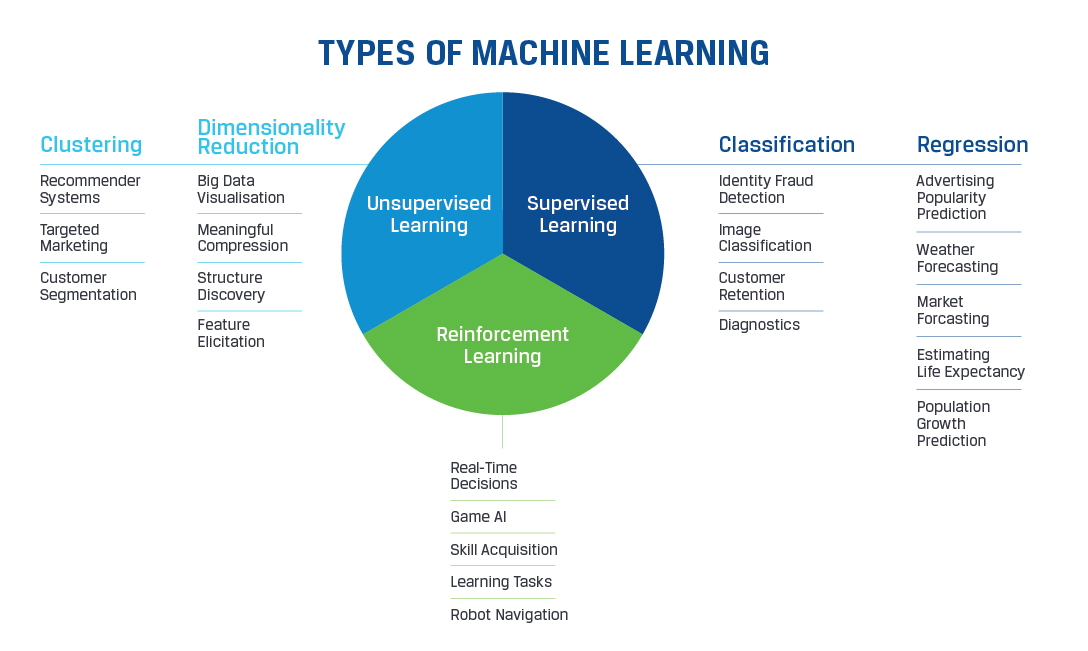
\includegraphics[width=\linewidth]{learning.jpg}
  \caption{tre maggiori tipi di learning\cite{learn}}
  \label{fig:ml}
\end{figure}
In figura \ref{fig:ml} vengono mostrate le tre maggiori classi. Nel contesto di questa tesi, siamo interessati esclusivamente al \textbf{Supervised Learning}, in particolare
ad algoritmi di \textbf{Deep Supervised Learning} basati su \textbf{Reti Neurali Convoluzionali}.
\subsection{Deep Supervised Learning}
La forma più comune di Machine Learning è il supervised learning. Consideriamo ad esempio il caso in cui si vuole addestrare un classificatore
che sappia riconoscere i diversi tipi di segnali stradali. Si colleziona un grosso dataset composto da immagini di segnali stradali, ciascuno di esso con la rispettiva categoria(stop, limite di velocità
divieto di sosta ecc.). Queste immagini compongono il \textbf{training set}. Durante l'apprendimento, vengono mostrate alla macchina  le immagini del training set. Per ciascuna immagine l'algoritmo produce un output della forma di un vettore di punteggi, uno per ogni categoria.
Si calcola una funzione che misura l'errore(o distanza) fra l'output prodotto e l'output desiderato. In base all'errore commesso l'algoritmo modifica dei paramentri interni, detti pesi, 
in modo da ridurlo. Per aggiustare il vettore dei pesi in modo corretto , l'algoritmo di apprendimento calcola un \textbf{vettore gradiente}, che indica, per ogni peso, la variazione dell'errore
causata da un piccola variazione del peso. Il vettore dei pesi viene aggiustato nella direzione di massima decrescita del gradiente. La fase di addestramento termina quando si raggiunge il minimo errore possibile, calcolato come la media della funzione di errore su ogni immagine del dataset.
Terminato il training, la prestazione del classificatore viene misurata su un differente dataset di immagini, detto \textbf{test set}. Questo serve a verificare
la capacità di generalizzazione della macchina, l'abilità di produrre output corretti anche su input sconosciuti.

\begin{figure}
  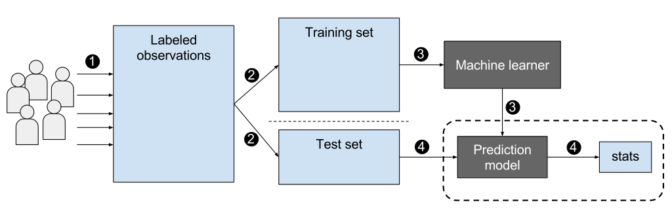
\includegraphics[width=\linewidth]{sup.png}
  \caption{Supervised Learning\cite{sup}}
  \label{fig:sup}
\end{figure}

Una grossa fetta delle applicazioni pratiche utilizza classificatori lineari su caratteristiche modellate a mano. 
Un classificatore binario calcola una somma pesata delle componenti del cosidetto \textbf{feature vector}. Se la somma è sopra una certa soglia, 
l'input è classificato in una certa classe. I classificatori lineari suddividono lo spazio degli input in semplici sottoregioni dette iperpiani, ma contesti come il riconoscimento di immagini o il riconoscimento vocale hanno
bisogno di modelli più complessi, capaci di rilevare  minuscole variazioni su caratteristiche importanti(\textbf{selettività}) e di ignorare anche grosse variazioni su caratteristiche irrilevanti al contesto, come ad esempio una rotazione dell'immagine(\textbf{invarianza}). La scelta delle caratteristiche rilevanti è quindi una
fase fondamentale del processo di learning. Tradizionalmente, la scelta delle features veniva costruita direttamente dagli sviluppatori, il che comportava una grande richiesta di abilità ingegneristica e di competenza nel dominio di lavoro.
Grazie al Deep  Learning  il processo di estrazioni di features rilevanti viene automatizzato con una procedura di apprendimento a scopo generale.
Un'architettura di deep learning è formata da uno stack multilivello di moduli elementari, tutti(o la maggior parte) sottoposti a learning, e la maggior parte dei quali
calcola una mappatura non lineare tra input-output. Ciascun livello aumenta sia la selettività che l'invarianza della rappresentazione. 
Maggiore è la profondità dello stack, maggiore è la complessità della funzione di scelta, capace di rilevare i più piccoli cambiamenti a dettagli rilevanti\cite{deep}.

\subsection{Reti Neurali}

\begin{figure}
  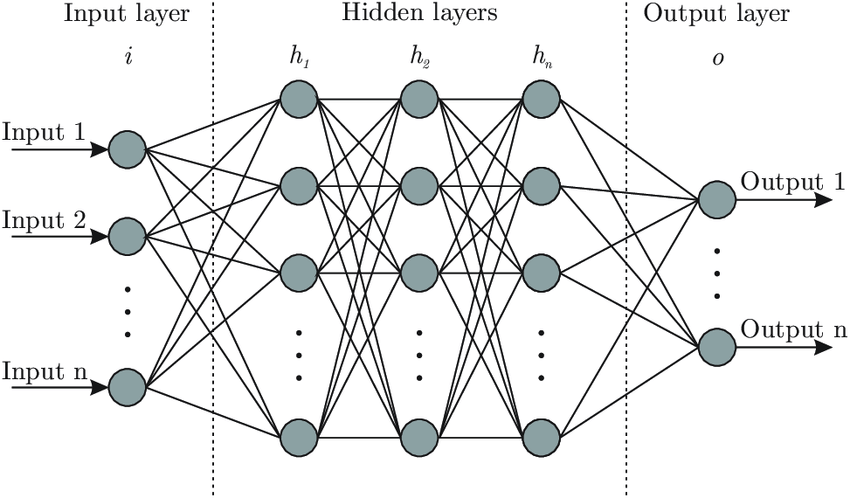
\includegraphics[width=\linewidth]{ann.png}
  \caption{schema base di una rete neurale\cite{ann}}
\end{figure}











    